\chapter{System Design and Implementation}

\section{Global System Design}
In this section, we will explain how we designed the application and why we made several decisions.
We do this with different diagrams.
We have made for example a class diagram, a database diagram, sequence diagrams and state diagrams.

\subsection{Database}
In Figure~\ref{database_diagram}, you see our database diagram.
We will explain the structure of the database shortly.

\begin{figure}[h]
    \centering
    \captionsetup{justification=centering}
    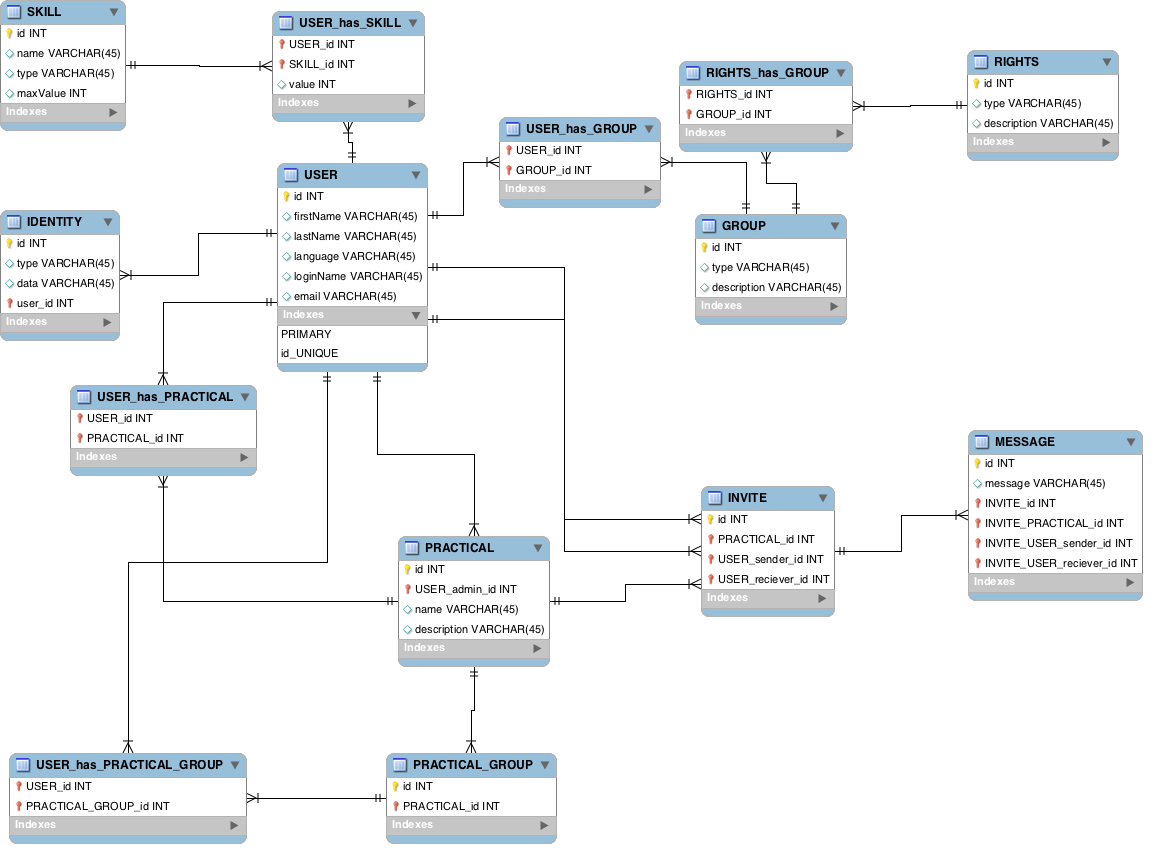
\includegraphics[width=\textwidth, frame]{images/database_diagram}
    \caption{The database diagram}
    \label{database_diagram}
\end{figure}

\noindent In the center of the diagram, you see the user.
The user has a many to many relation with a group.
There are four different groups.
There is a group for students, for teachers, for administrators and one for guests.
It is obvious that a group can contain multiple users, but a user can also have multiple groups.
Users can be a teacher, as well as an administrator.

Every group has different rights.
The same right can also be assigned to multiple groups.
That is why we also have a many to many relation between a group and a right.
\\\\
A user must also be able to log in.
To accomplish this, the user must have an identity.
An identity can only belong to one user.
If this should not be the case, the system would not be save because other users have access to a user's rights.
\\\\
A user can be part of multiple practical groups and a practical group consist of multiple users.
Therefore, user and practical group have also a many to many relation.
This is the same for user and practical.

A practical group belongs to only one practical.
A practical group does not belong to multiple practicals.
\\\\
An invite has two many to one relations with a user.
An invite has a sender as well as an receiver.
There can only be one sender and one receiver for an invite.

Every invite belongs to only one practical.
These therefore have also a many to one relation.
\\\\
The last relation is between an invite and a message.
These messages are for communication between the sender and the receiver of the invite.
An invite can have multiple messages.
Every message belongs to only one invite.

\subsection{Class Diagram}
In Figure~\ref{class_diagram} you can see our application's class diagram.
This diagram is not complete with all the methods and attributes, but the most important methods and attributes are included.
For example, all the get and set methods are not included.
\\\\
The structure of this diagram looks a lot like the database diagram.
In this diagram, we make a difference between a student and a user, because they can perform different actions.

For example, only a teacher can create courses.
A student cannot do this, a student can only sign up for this courses.
\\\\
A student can also find possible group members.
These possible group members are determined by the recommender class.
With the getNextGroupMember method the next best practical partner will be calculated.
You can read more about the matching algorithm in Section~\ref{sec:algorithm}
\\\\
The other methods are needless to explain.
The name of the methods tell the function.

\begin{figure}[H]
    \centering
    \captionsetup{justification=centering}
    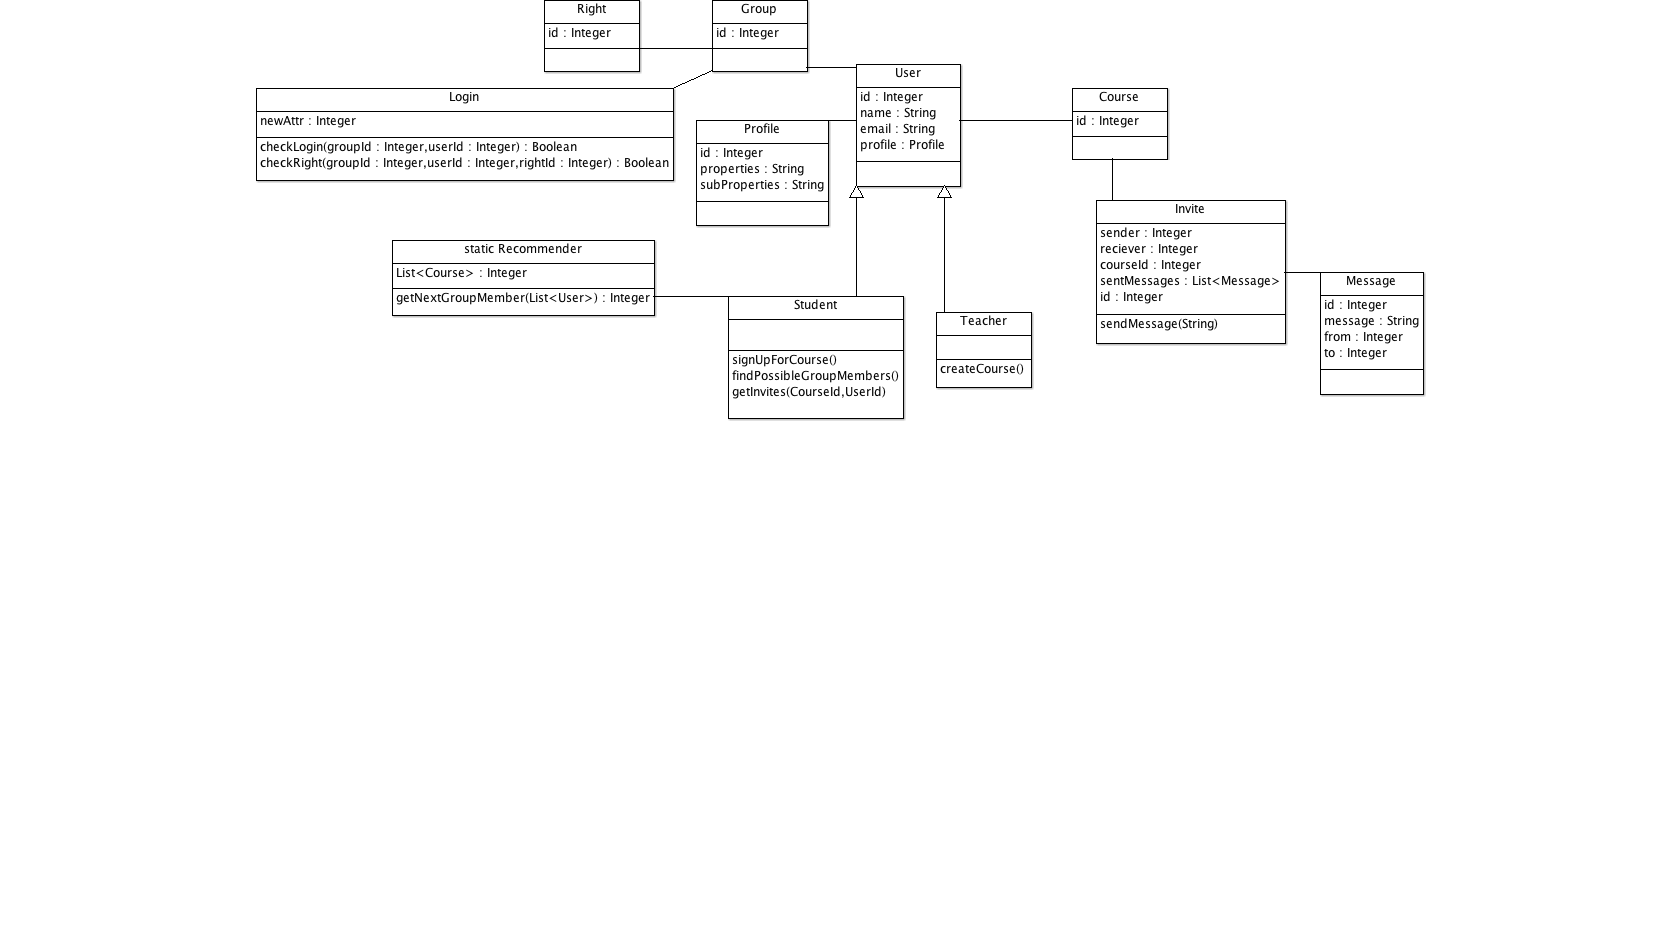
\includegraphics[width=\textwidth, frame]{images/class_diagram}
    \caption{The class diagram}
    \label{class_diagram}
\end{figure}

\subsection{State Diagrams}
In this section we describe the behaviour of our system with the help of state diagrams.
We describe this behaviour with two different state diagrams.
One diagram for the administrator and an other one for a student.
\\\\
First of all, the administrator must be registered and logged in before he can perform any action.
When the administrator is logged in, he can create practical.
When the practical is created, the administrator can manage this practical.

One of the parts of managing the practical is managing the users that are enrolled for this practical.
The admin can remove users or even entire practical groups.

\begin{figure}[H]
    \centering
    \captionsetup{justification=centering}
    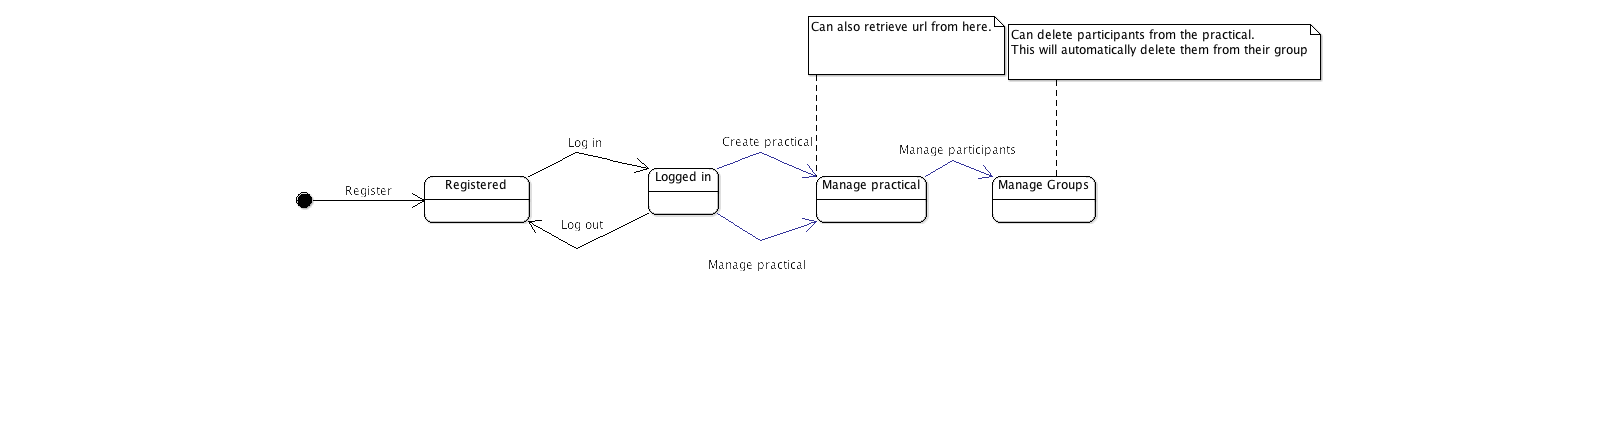
\includegraphics[width=\textwidth, frame]{images/state_diagram_admin}
    \caption{The administrator's state diagram}
    \label{state_diagram_admin}
\end{figure}

\noindent The student's state diagram is a little bit more complex.
The first part is the same as with the administrator.
The student also must be registered and logged in to perform any action.
\\\\
When the student is logged in, he has an option.
He can either go to his profile, or manage his practical.
When he chooses to go to his profile, he can view or edit it.
\\\\
The courses have some more options.
First of all, the student can see which fellow students are recommended to join his group.
The student can invite these students to join his practical group.

The student can also view the overview of his invites.
This overview includes both received and sent invites.
When the student accepts an invite, both the practical groups are joined.

\begin{figure}[H]
    \centering
    \captionsetup{justification=centering}
    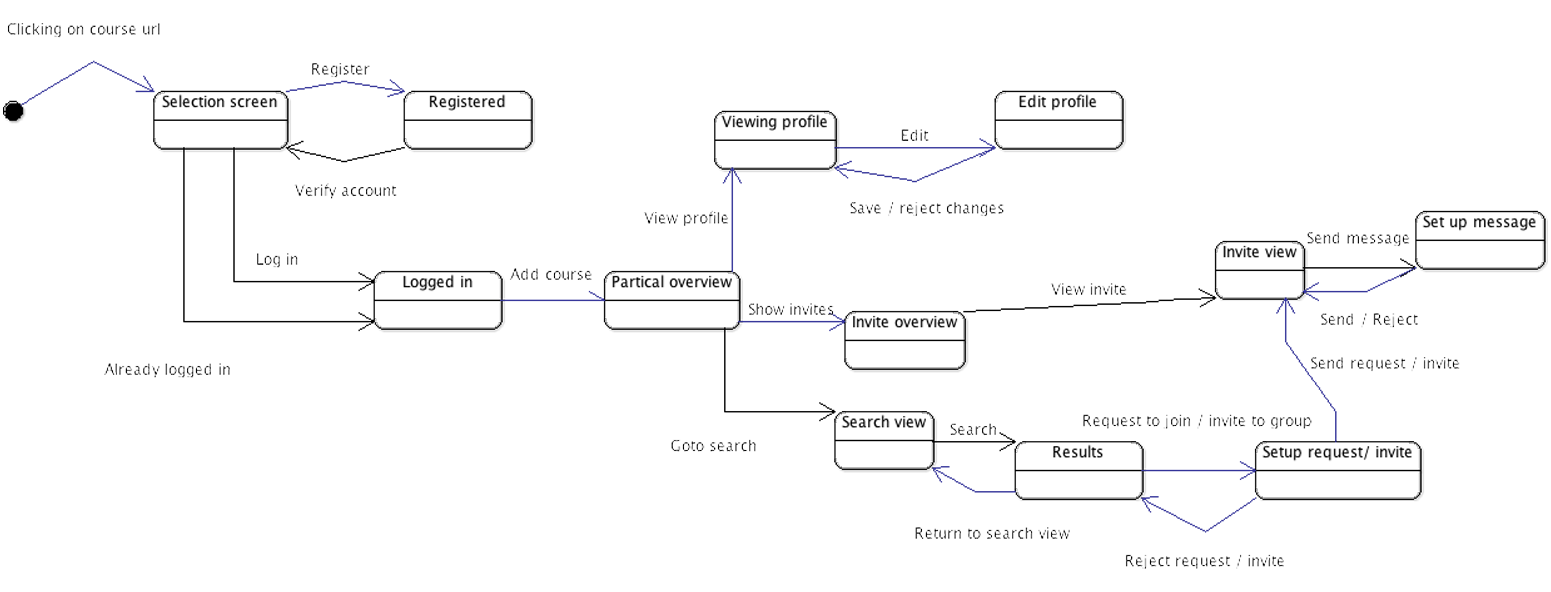
\includegraphics[width=\textwidth, frame]{images/state_diagram_participant}
    \caption{The participant's state diagram}
    \label{state_diagram_participant}
\end{figure}

\subsection{Sequence Diagrams}
In this section we explain the sequence diagrams.
We have only made a sequence diagram for logging in, but because of the Model View Controller structure (Section~\ref{sec:mvc}) most of the actions have a similar sequence diagram.
\\\\
The user only has direct contact with the views.
The views send the information that the user provided to the controllers.
After that, the controllers collect the required information from the database via the models.
\\\\
When the controllers have all the required information, they execute their calculations.
After the calculations are fully executed, the results will be sent back to the views.
The views display these results and via these views the results will reach the users.

\begin{figure}[H]
    \centering
    \captionsetup{justification=centering}
    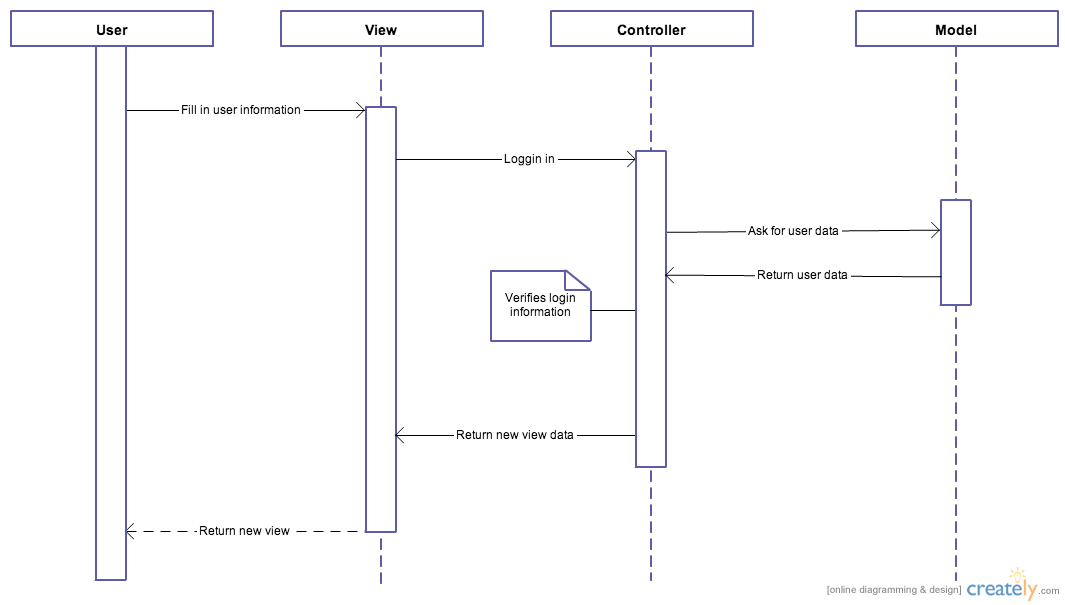
\includegraphics[width=\textwidth, frame]{images/sequence_login}
    \caption{The sequence diagram for logging in}
    \label{sequence_login}
\end{figure}

\section{Model View Controller}
\label{sec:mvc}
As mentioned earlier, we are using the Play Framework. 
This frameworks follows the Model View Controller (MVC) architectural pattern applied to the Web architecture\cite{playframework_mvc}.
This pattern splits the application into separate layers: the Presentation layer and the Model layer. 
The Presentation layer is further split into a View and a Controller layer.

\subsection{Controller}
The \textbf{Controller} responds to events (typically user actions) and processes them, and may also invoke changes on the model.
In a Web application, events are typically HTTP requests: a Controller listens for HTTP requests, extracts relevant data from the 'event', such as query string parameters, request headers... 
And applies changes on the underlying model objects.
\\\\
In Play, a Controller is a Java class where each public, static, method is an \textbf{action}.
An action is a Java entry point invoked when a HTTP Request is received.
The Java code from the Controller class is not really object oriented: it is mainly procedural code.
The action method extracts relevant data from the HTTP request, reads or updates the model objects, and sends back a result which is wrapped into an HTTP Response.

\subsection{Model}
The \textbf{Model} is the domain-specific representation of the information on which the application operates.
Domain logic adds 'meaning' to raw data (e.g., calculating if today is the user's birthday, or the totals, taxes, and shipping charges for a shopping cart).
 Most applications use a persistent storage mechanism such as a database to store data.
MVC does not specifically mention the data access layer because it is understood to be underneath, or encapsulated by, the Model.
\\\\
In Play, the domain model object layer is a set a Java classes using all the object oriented features available from the Java language. 
It contains data structures and operations on which the application operates. 
Whenever model objects need to be saved into a persistent storage, they may contain some glue artefacts like JPA annotations or SQL statements.

\subsection{View}
The \textbf{View} renders the model into a form suitable for interactions, typically a user interface.
Multiple views can exist for a single model, for different purposes.
In a Web application the view is usually rendered in a 'Web format' like HTML, XML or JSON.
However there are some cases where the view can be expressed in a binary form, e.g. dynamically rendered chart diagrams.
\\\\
In Play, most of the application views are generated using an efficient template system provided by play. 
The Controller gets some interesting data from the model layer, and then applies a template to decorate these objects. 
This packages contains HTML, XML, JSON and other template files with special directives used to dynamically generate the model representation.
\\
\begin{figure}[h]
  \centering
    \captionsetup{justification=centering}
    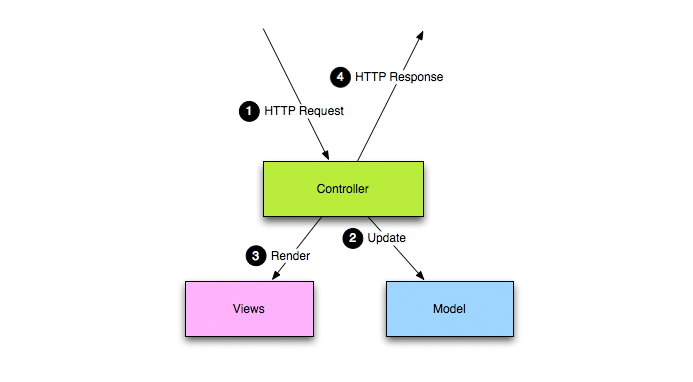
\includegraphics[width=\textwidth]{play_mvc}
    \caption{Play Framework MVC structure}
  \label{play_mvc_image}
\end{figure}


\section{Implementation}
In this section we will describe the software implementation of APMatch.
We will start of with some global implementation description of our APMatch system and then we will continue with some more advanced topics.

We chose to explain some more about both the invites and the matching algorithm.
For the invites we explain what are difficulties were and which situations were hard to implement, while for the matching algorithm we will explain some more how it works and why we chose it.

\subsection{Global}
During the implementation we chose for the git feature workflow as described in section \ref{software_development_method}.
Most of the time this lead us to small and nice feature's which added both the model as well as the visuals to the APMatch system.
There were some exceptions like the Invites and Matching algorithm which were a lot harder to implement than expected.
These big feature's sometimes broke our workflow, because there were too many dependencies between the different features.
Luckily most of the time there were enough other feature's that could be implemented to solve the issue of waiting on the dependencies to be implemented.

Our global implementation went as planned and made use of the MVC design method of the Play Framework.
This lead to a nice structured way of models that related closely to the database model, containing most of the functionality of the APMatch system.
We also extended the MVC model a bit with a helper package which contains functionalities like hashing, Linkedin and the matching algorithm.
The helper classes don't relate to the database model, but will supply the needed functionalities for the controllers.

The controllers of the of the MVC model were defined in six different controllers: Application, Authentication, Invite, Practical, PracticalGroup and Profile.
The Application controller only provides the static pages like the home page, contact page and the information page.
The Authentication controller provides the functionalities for both the Linkedin login, and the normal authentication and registration.
All the other controllers provide the functionality for all the pages which relate to the subjects of their name.

\subsection{Invites}
One of the most underestimated parts of the implementation of APMatch was the invites system.
This part took by far the most time during the implementation phase, but was at firs estimated as a part which could be quickly implemented.
This underestimation was mostly caused by the complexity of the invites system, which we will explain in the following paragraphs.
After that we will explain how we solved this difficult invite system, and conclude with what could be improved to make it even better.

So why is this invite system so complex?
This all is mainly caused by the problem that occurs when creating practical groups larger than two.
Creating a group larger than two requires either a group manager to create and maintain invites, or a different way of inviting people when you are joined in a practical group.
This is needed because of the fact that having the possibility for all the group members to invite other people could lead to several conflicting situations.
So the easiest way to solve this is by creating a group manager, which would be the only user that has the rights to send and invite other users.

But then how do we chose a group manager?
We could of course easily solve this by doing it random, but that could lead to strange situations and then you also need to add group manager functionalities, to for example change the group manager.
To avoid these situations we then chose to instead of doing it random, make the inviter that forms the group the group manager.
This will make it sure that when you accept a certain invite you also know who will be the group manager and also can depend your choice on that.

Despite the fact that we now solved both the complex system of having more then two group members, there were still other problems that also caused our underestimation.
This was due the fact that you could have multiple open invites available at a certain time, both send invites and received invites.
Here we could have chosen to deny the user to have multiple outstanding invites to users, but because we expect that there will be a lot of inactive users this seems very implausible.
Users will then have to wait a certain amount of time for an inactive user, while other possible groups members might join other groups.
This is why we chose to implement it that when an invite is accepted and you're not becoming a group manager, all the other invites will be rejected.
Hereby the problem of having multiple open invites at a certain time is solved.

One of the last problems we found during the implementation of the invites system was the fact that you should be able to invite a group.
This caused two different subproblems, one person inviting a group and a group inviting another group.
Both were dealt with in the same way, by defining that a single person is also a group with just one person in it.
This only left us with the merging of two groups which was done the same way as joining one by one.

Because of all these all these edge cases we needed to test the invite system very carefully using a lot of unit tests.
Finding these edge cases, defining the edge cases and then writing the unit tests for these edge took more time than expected.
Initially we didn't taught of all these edge cases and were just thinking of a simple invite system.

For the future we advise to first think out the whole invite system and split it up in smaller features.
Then both the progress will be easier to track and writing tests cases will also be easier.
We also advise to make it more understandable for the user what exactly is happening during the invites.
This means that the users needs to know what happens to his other invites when he for example accepts an invite.
Also hiding the fact that the user is in a practical group on its own should make it more understandable for the user what is happening with the invites.

\subsection{Matching algorithm}
\label{sec:algorithm}
For our matching algorithm we used our custom designed algorithm.
This algorithm uses the skills defined by the user and the teacher to find the best matching with the preferences of the teacher.
We will first give a description of the algorithm followed by a formal description.
After that we will give a description about the complexity and will conclude this section with why we chose this implementation.

Before we start explaining the algorithm we will first describe how to calculate the distance for a certain practical group.
Calculating the distance of a practical group is done by going through the skills defined by the practical teacher.
We will then calculate the average of the values of the skills of all the users in the practical group and the users' practical group combined.
Then all the average's are multiplied with each other and then you take root of the amount of skills in the practical.
This resulting number will defined as the distance.

The matching algorithm starts with a practical and user.
It will start with going through the different practical groups in the practical.
To simplify the algorithm it is chosen to make sure every user is in a practical group.
This means that when an user doesn't have any practical partners he is still in a practical group with only himself in it.
While going trough the different practical groups it will calculate the distance as described in the previous paragraph.
After calculating the distance with every other practical group and saving this in a map, this result is sorted by descending distance.
Then we start recommending practical groups to the user starting by the top of the list.
The formal definition of this algorithm is visible in Algorithm \ref{recommend}.

\begin{algorithm}
\begin{algorithmic}
\Function{Recommend}{$practical$, $user$}
	\State $resultList\gets$ Empty map of PracticalGroup and distance
	\ForAll{$practicalGroups$ in the $practical$}
		\State $distance\gets 0$
		\ForAll{$skills$ in the $practical$}
			\State $average\gets 0$
			\ForAll{$users$ in the $practical$}
				\State $average\gets average + SkillValue(user, skill)$
			\EndFor
			\ForAll{$users$ in the $user$ practical group}
				\State $average\gets average + SkillValue(user, skill)$
			\EndFor
			\State $average\gets average / (amount\_of\_users)$\Comment{The amount of users in the practical}
			\State $distance\gets distance * (average - SkillValue(Practical, Skill))$
		\EndFor
		\State $distance\gets distance ^ {(1 / amount\_of\_skills)}$\Comment{The amount of skills in the practical}
		\State $resultList\gets resultList + (practicalGroup, distance)$
	\EndFor
	\State Sort the $resultList$ by descending $distance$
	\State \textbf{return} $resultList$
\EndFunction
\caption{The recommendation algorithm}\label{recommend}
\end{algorithmic}
\end{algorithm}

To Analyse the complexity we need the following measurements.
We define $n$ as the amount of practical groups in a practical.
We define $m$ as the amount of skills defined in a practical.
We define $j$ as the amount of users in a certain practical group plus the amount of users in your own practical group.
Since in the first loop we go trough the practical groups to calculate the distance we start with a time complexity of $O(n)$.
Inside this loop we go trough each of the skills defined in the practical to calculate the average which will give us $O(n*m)$.
In order to calculate this average we need to go rough all the users in our practical group and the practical group examined.
This will lead to a time complexity of $O(n*m*j)$.
As one of the last steps we still need to sort the list of the practical groups which will be done in a time complexity of $O(n*log(n))$.
All this combined will lead into a total time complexity of $O(nmj+n*log(n))$ which for small $m$ and $j$ will lead to a total time complexity of $O(n*log(n))$.

We chose this implementation, because it is very easy to understand and very adjustable implementation of the algorithm.
There are several ways to optimise the algorithm by using precomputing.
This can be done for example during the defining of the skills by the user and will save execution time when viewing recommended solutions.
Next to that we have shown in the previous paragraph that with both a small amount of skills defined by a practical and with a small amount of users in practical groups, this algorithm will run in $O(n*log(n))$.
Since this will be the case, because both sizes are limited this will be fast enough to run while recommending without precomputing.
All these cases prove that the algorithm is good enough for recommendation system.



